\documentclass{article}
\usepackage{graphicx}
\usepackage{geometry}
\geometry{margin = 3cm}
\title{Information visualization}
\author{Ari Viitala}
\begin{document}
	\maketitle

\section*{Exercise 1}
Yes.
\section*{Exercise 2}

In this exercise we have investigated the marital statuses of people of Helsinki in the year 2004. The dataset has been obtained from Helsinki regional info share and contains the marital statuses of all people who resided in Helsinki in between year 2004 and 2017 but here we have only considered the year 2004 in our analysis. People in the dataset have been divided into four categories single (from the perspective of Finnish law), married, divorced and widowed. People have been grouped by age every 5 years from age 0 up to the age of 95 and for each segment the amount of people in different marital categories has been reported.

In the figure \ref{absolute} we can see the absolute values of people in each category for all ages and for both women and men. We can clearly see that the amount of married people remains understandably zero until close to age 20 since the legal marrying age in Finland is 20 years. We also see a big leap in total population during this time. Helsinki has Finland's largest university and a lot of jobs so there is a large inflow of young people which explains the population almost doubling between the ages 20 and 30. During this time we also see a rapid increase in the amount of married people as well as an increase in divorced people following a bit later bit behind. At this point the total population also starts to drop as it is common to move to the neighboring communities for cheaper accommodation when starting a family becomes topical. 

At this point the amount of married people seizes increasing but divorces continue rising at a steady pace and the amount of single people continues to fall also at a steady pace. Around the age of 60 there is a bump in the total population which is explained by the "large generations" who were born right after the war and at 2004 were around 60 years old. From this point on we see a rapid decline in population for both genders which also leads to amount of married and divorced people to rise. Also here we arrive to the biggest difference in the graph between the genders, the widowed line which is depicted with the dotted line. For men this line is barely visible above the x-axis but for women there is a clear increase which easily overtakes all the married, divorced and single populations. This effect is largest around the 80 year mark and I can think of two possible explanations. 

The clear explanation is that the average life expectancy for men in Finland is a couple of years shorter than for women due to unhealthier life styles as well as being more prone to accidents. However men born in early 1920's were also the ones killed the most during the war years 1939-1945 so this could also be a cause for such a large increase in the amount of widowed people. In the description of the dataset it is not explained how people are classified if they re-marry but I would assume that they would be reclassified as married which would be the most probable scenario for women who lost their husbands in the war.

 
 
\begin{figure}[h!]
\centering
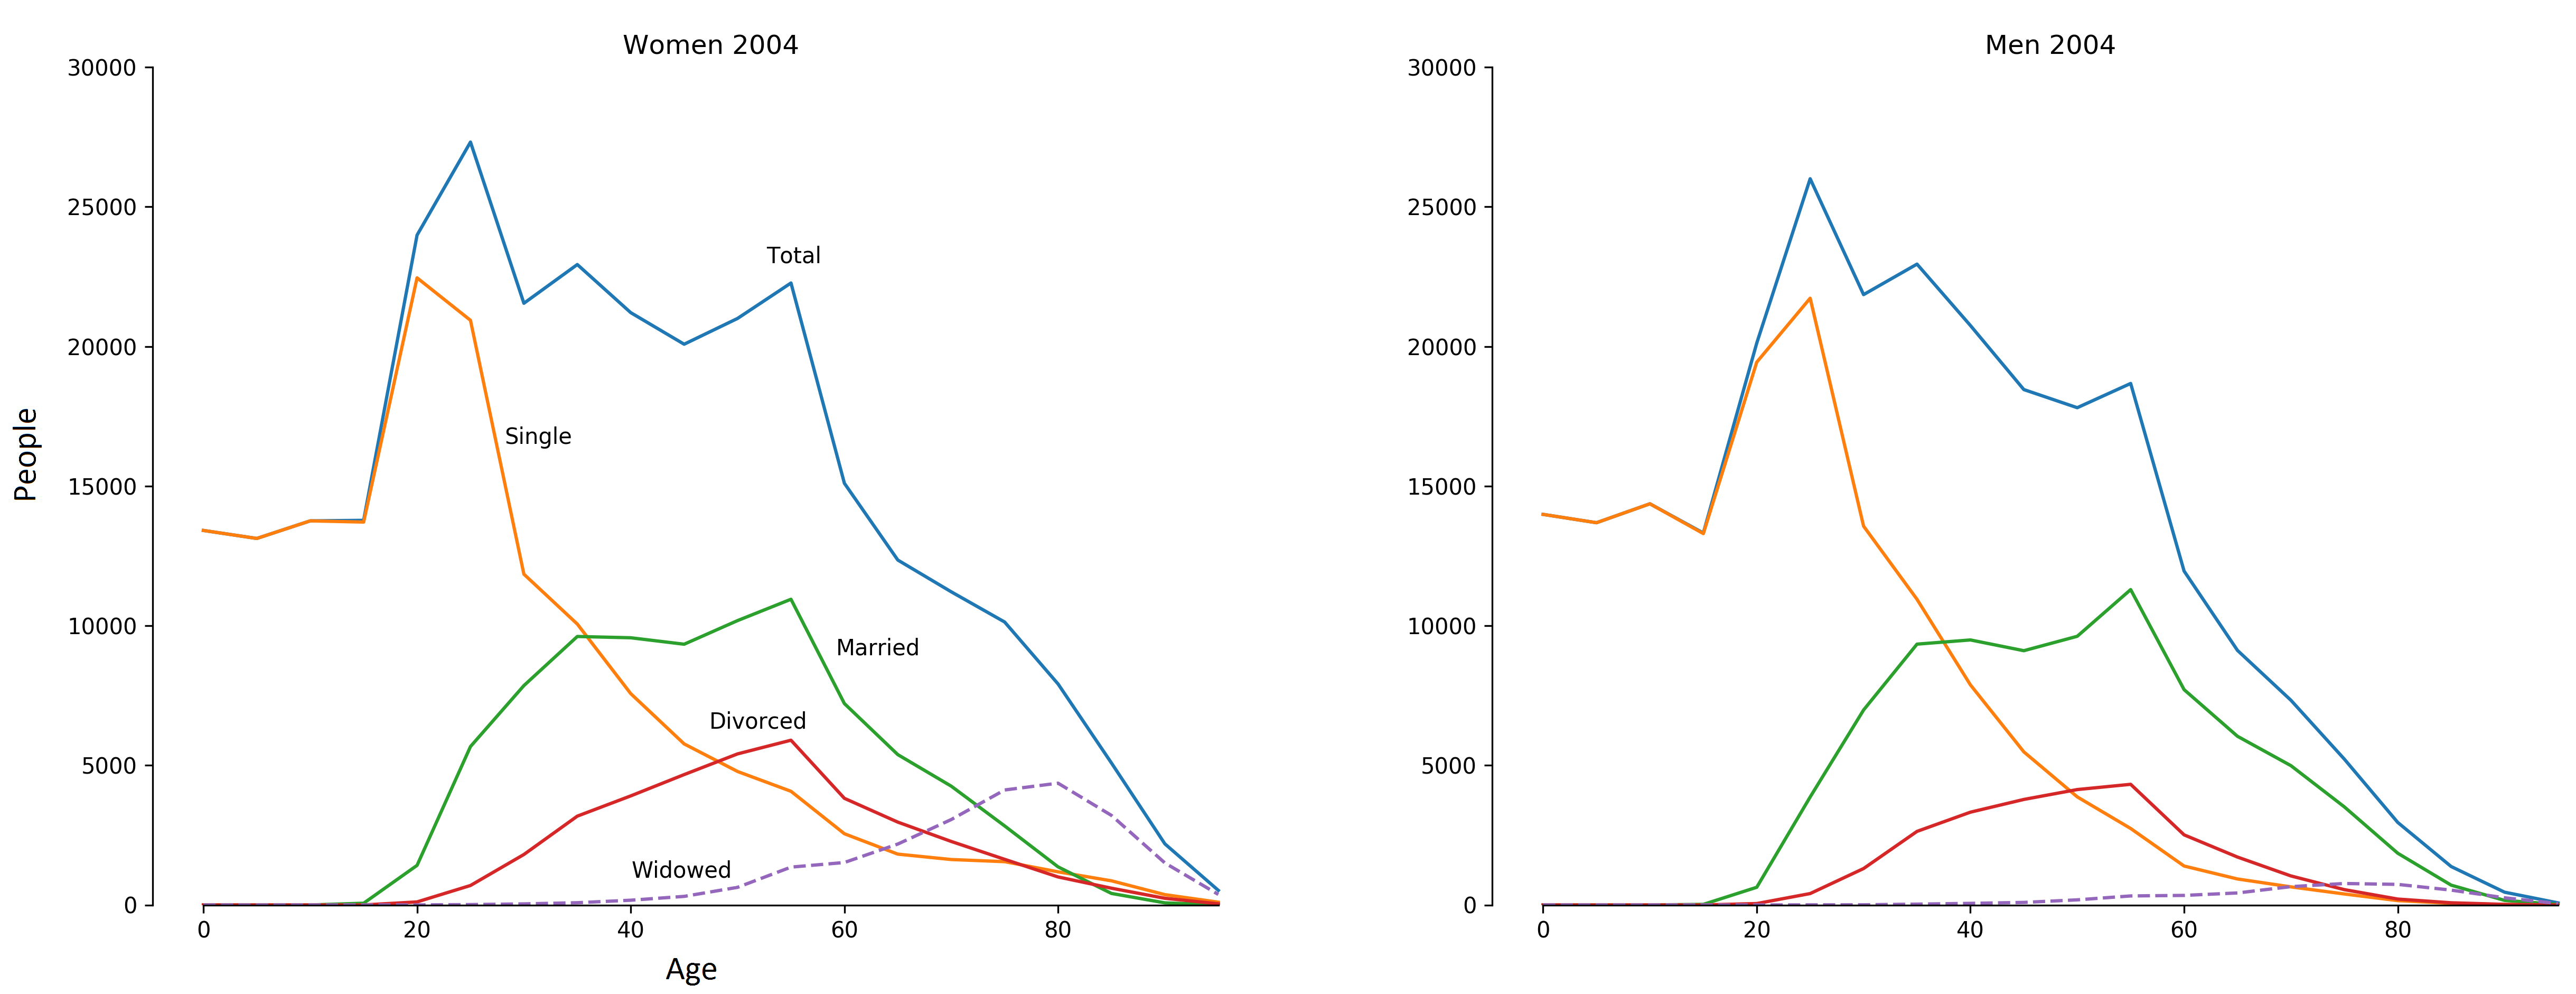
\includegraphics[width = \linewidth]{absolute}
\caption{Marital statuses of women and men in Helsinki in the year 2004.}
\label{absolute}
\end{figure}

Even though the absolute sizes of different age groups are descriptive on their own accord, deciphering differences between the relative sizes of the marital groups can be a little difficult. In figure \ref{relative} it plotted how the marital groups' relative sizes change as a function of age. This also brings out new differences between age groups that were near impossible to see from just the absolute size graph especially in the latter years where the age groups are smaller and dwarfed by the larger age groups. 


One thing we immediately see from this graph is that men are much more likely to be married in their sixties to eighties than women. The percentage of men who are married during this time period is  nearly 80\% but for women the corresponding number is about 50\%. This could either suggest that divorced, single and widowed men die faster than their married counterparts which would lead to an increase in the relative size of married men. One other explanation would be that men are more prone to remarrying younger women which would also increase the amount of married men. However, it is more probable that marriage is beneficial for men's health as or married men are generally more healthy thus stay alive longer. 

One other thing we notice that significantly larger portion of women never marry and again this would have been much harder to distinguish from the absolute value graph. During the latter years the portion of women who have never married is twice as large as the corresponding man's value. It would also seem like women who decide not to marry end up living longer than other segments as their relative size increases with time. One could argue that marrying is beneficial for the health of men but not marrying is beneficial for womens health. 

One last thing we can see from this graph is that women who are 90 years or older are really unlikely to have a husband the probability being close to zero. The situation is completely different for men however. Out of 95+ year old men nearly a third are married. This would suggest that women are more likely to outlive their partners up until the very end. 

\begin{figure}[h!]
	\centering
	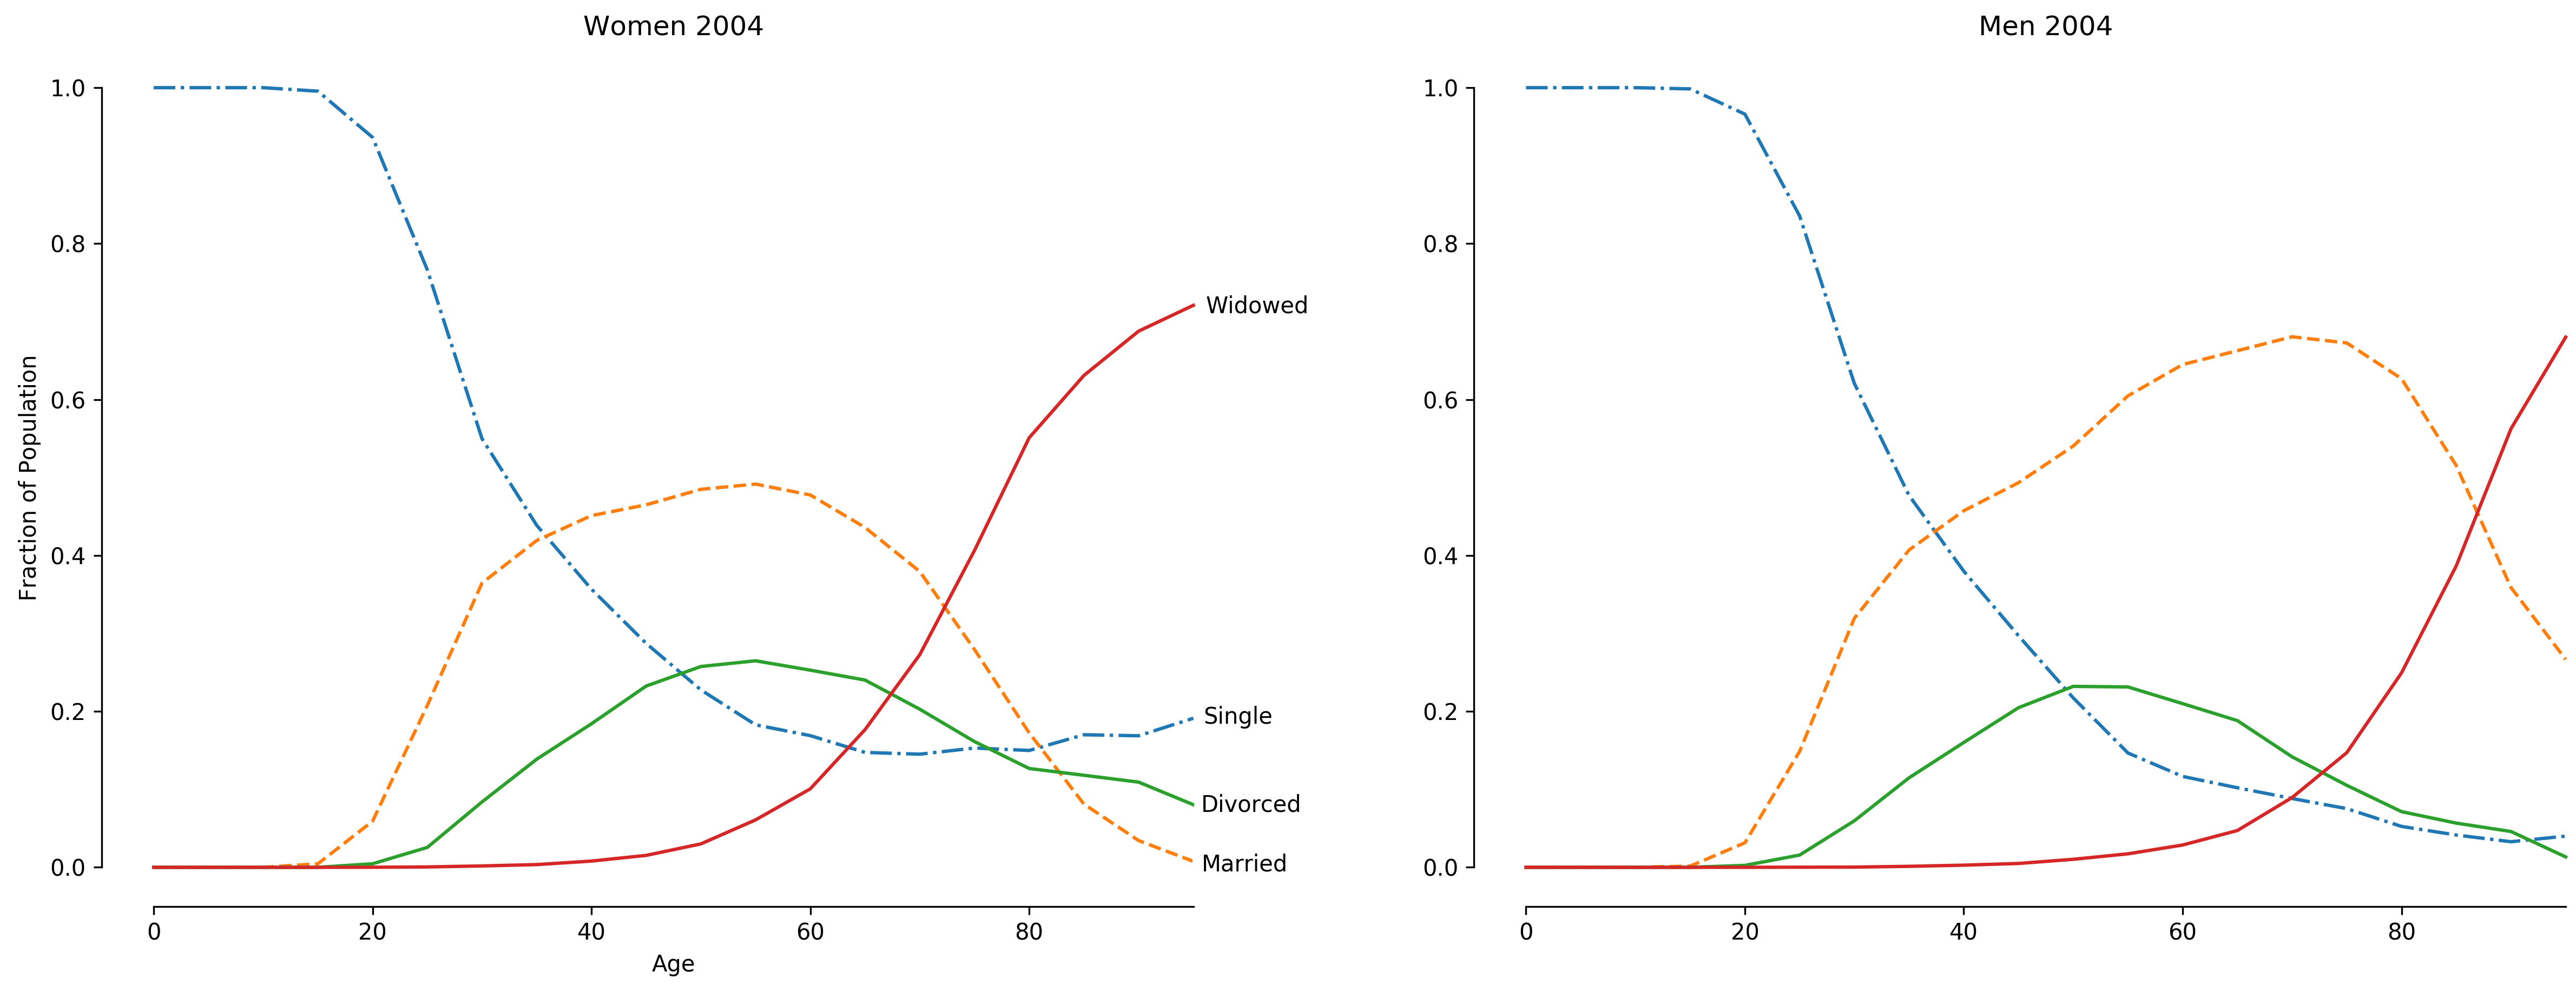
\includegraphics[width = \linewidth]{relative}
	\caption{Relative amount of women and men with different marital statuses in Helsinkin in the year 2004.}
	\label{relative}
\end{figure}

In figure \ref{cumulative} it has been plotted how the different marital groups form the whole population as a function of age relative to the total size of the group. Here the whole population both, men and female, is considered.

This visualization captures, in my opinion, the evolution of different groups really well. Around the 20 year mark the marriage starts eating away at the single people segment and by the year 60 there has been established a certain division between people who marry and people who will never marry. As time goes on the divorced segments starts chipping away from the married segment and reaches its's maximum by age 50 and then starts diminishing probably because people remarry. By the seventy year mark there has been established a certain segment of people who have been married and divorced and never remarried again and this then stays constant for the rest of the age groups. Then there is the widowed segment that begins gaining ground at the 50 year mark and as time goes on increases with accelerating speed. This graph is also a bit sad since it seems that if you reach the age of ninety it is really improbable that you are happily married since the married segment is dwarfed by those who never married, divorced or ended up as widows. 

All in all the dataset proved to be pretty interesting and offered surprising results like the big bump in amount of widows in women seen in figure \ref{absolute} and the much higher percentage of married men in their 70's and 80's compared to women which could be brought out with some clever visualization. 

\begin{figure}[h!]
	\centering
	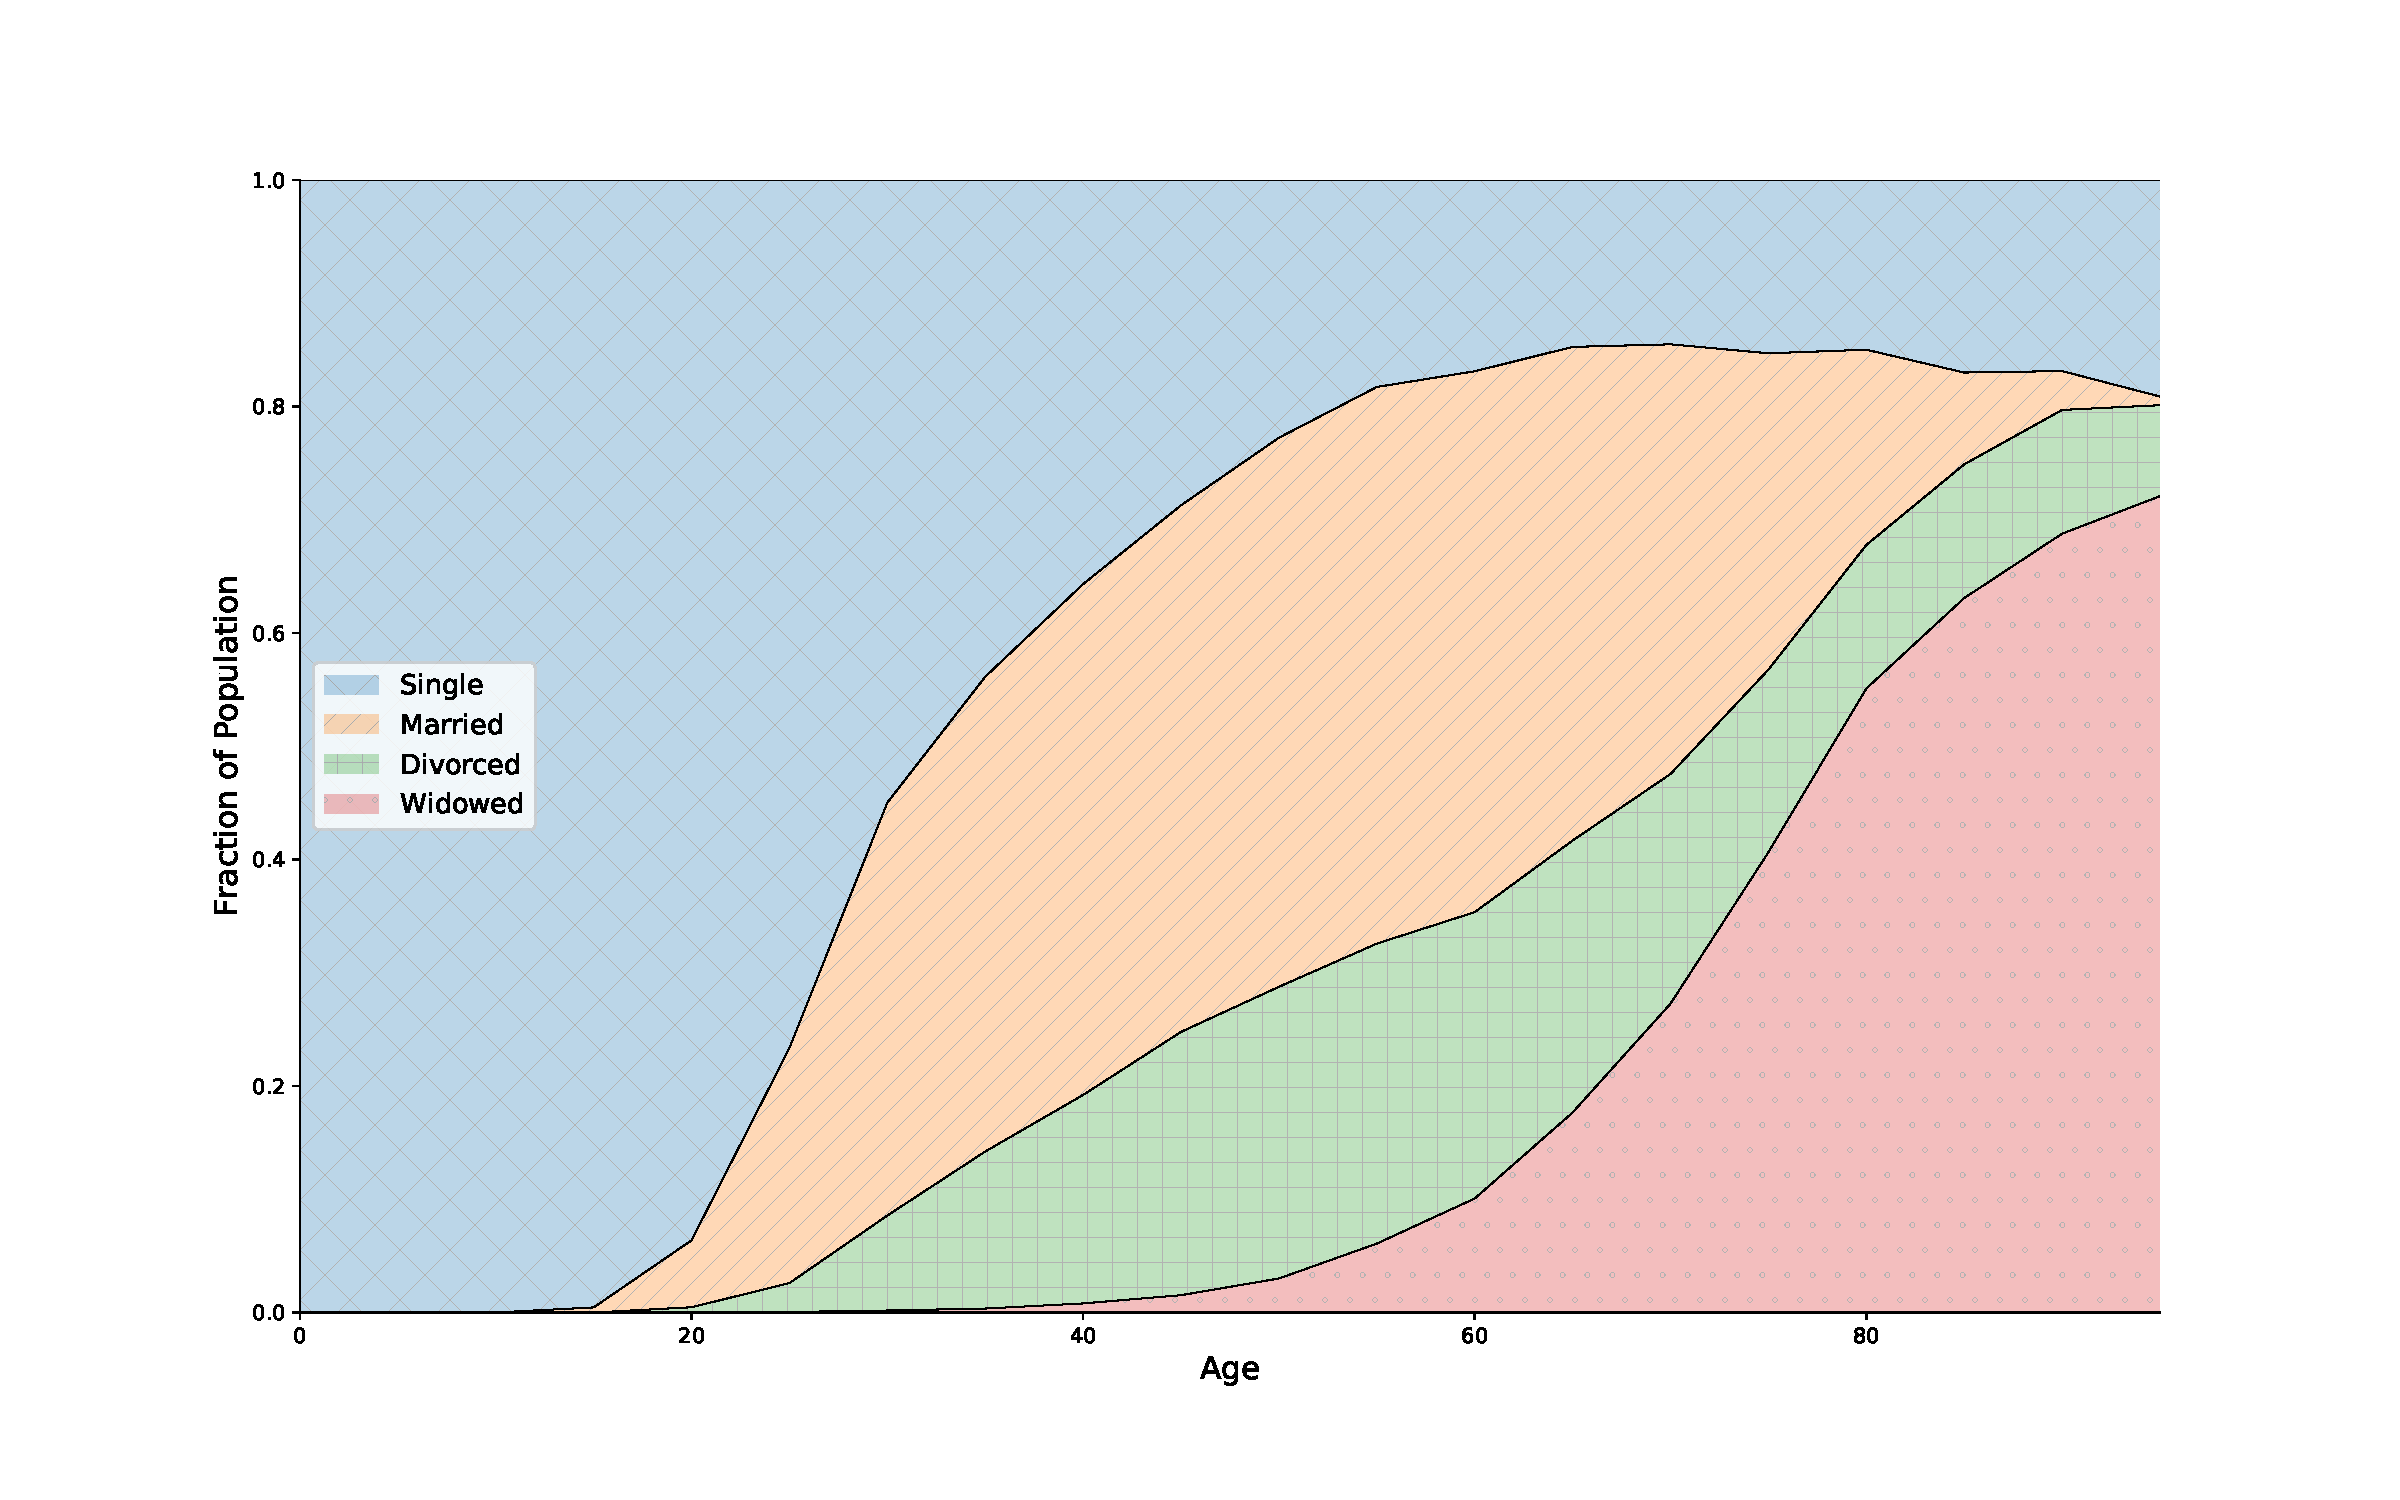
\includegraphics[width = \linewidth]{cumulative}
	\caption{Relative sizes of marital status groups as a function of age.}
	\label{cumulative}
\end{figure}

\newpage

\section*{Exercise 3}

The phenomenon where the gray line on darker background looks lighter than the one on the lighter background can be explained by how the human eyes ganglion cells that receive light impulses are organized. The cell consist of an inner circle that sends more pulses as it receives light and an outer circle that sends less pulses when it receives light. This means that the light received by the outer circle inhibits pulses that are created when the inner circle receives light.

When there is a steep gradient in the shade of color, the inner and outer circles receive different amounts of light. For example in the case of the gray strip on darker background when he inner circle cells receive light from the gray area and the outer cells receive impulse from the darker area when vision is focused around the edge of the strip. The outer cells inhibit signals sent by the inner cells less since they receive less light and this means that the shade of gray appears lighter. The effect is reversed in the light background case where outer cells receive more light and thus inhibit the signal more making the gray appear a darker shade.

The Difference of Gaussians model must be kept in mind when designing color scales because it alters how humans perceive changes in the lightness of colors. This means that the absolute shade of the color in the scale is not the only thing that contributes to how information is perceived. Also the intensity of the shades around it affect the value communicated. In practice this would mean that lightness scale cannot be solely trusted when delivering information but if we want to be sure that the message is perceived as we want it to we should avoid combining similar shades of the same color with varying backgrounds. Instead we should either avoid steep changes in gradient of find another way of conveying information than the shade of the color. 

\newpage
\section*{Exercise 4}

White balance setting is needed because the distribution of light is different based on the light source. Outdoors the light from the Sun contains more blue photons than light from for example light bulb or a fluorescent lamp. Human brain and eye can adjust to different distributions of photons pretty easily whereas a camera cannot. This can be seen for example in night mode filters for computer screens which filter out blue light. At first when the filter is applied the image color balance looks weird but after a while the image starts to look normal again as the brain adjusts to the new type of light.

The digital camera sensor is different to the human eye as it just counts the amount certain energy of photons hitting it. If all images were saved as raw images with just the counts and energies of the photons everything would be fine as the color balances could be adjusted such that it looks right to the human eye. 

Raw images, however, require a lot of space and that is why normally digital images are compressed. In this compression lies the problem since the compression algorithm needs to interpret the raw data such that it matches how the human brain would interpret that photon distribution. For example outdoors blue light would have to be suppressed in order to correct the image to match human perception and outdoor mode does exactly this. This is why, if we use the outdoor mode indoors, the blue light is over suppressed and the image becomes red. Vice versa, if indoor mode is used outside, blue light is not suppressed enough and the photo ends up being blue.

\newpage 

\section*{Exercise 5}  

In figure \ref{glyphs} is presented the asked glyph. The glyph can represent four variables with it's size, shape, color and the shade or deepness of the color. Out of these the size of the glyph and the deepness of the color can be continuous if desired. Shape and color are discrete and they can also be extended outside the set presented here. 

I think all of the variables are pretty easy to distinguish but if the glyph size gets small then maybe round and hexagonal glyphs can become a bit difficult to distinguish. Also the darker colors can be harder to distinguish in the extremes they are all more or less black or white when we get to really dark or light shades. 

Where my glyph might not be so great is the distinguishing of different sizes between different shapes. Humans are pretty bad at estimating area and are much better at seeing differences in length. This means that the dominant factor in the glyphs size dimension might not be the area but instead the height of the glyph. This is not necessarily a problem if the glyph is used such that only similar shape glyphs are compared or the visualization is designed such that the sizes are discrete or in some other way that there is no chance of ambiguity.
\begin{figure}[h!]
	\centering
	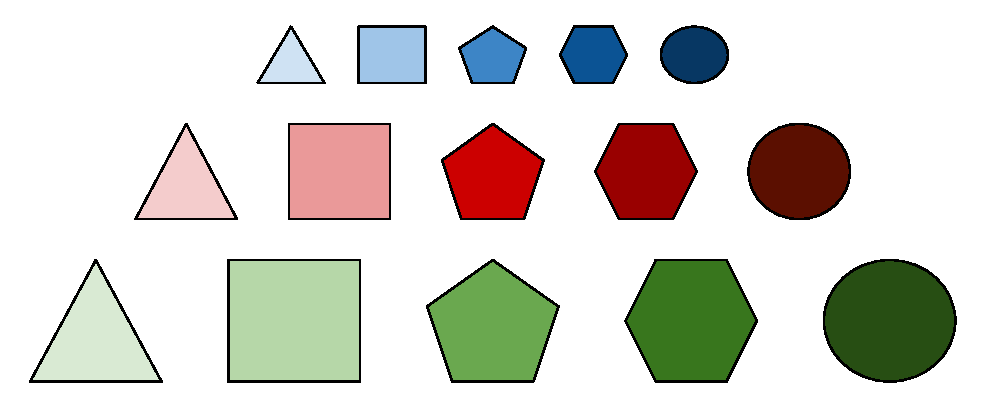
\includegraphics[width = \linewidth]{glyphs}
	\caption{A glyph set that is capable of representing four variables}
	\label{glyphs}
\end{figure}

\end{document}